\documentclass{article}

\usepackage[utf8]{inputenc}
\usepackage{graphicx}
\usepackage{amsmath}
\usepackage{amsfonts}
\usepackage{amssymb}
\usepackage{comment}
\usepackage{gensymb}
\usepackage{geometry}
\usepackage{float}
\usepackage{caption}
\usepackage{subcaption}
\usepackage{listings}

\geometry{a4paper, margin=1in}

\lstset{
    basicstyle=\ttfamily\small,
}

\title{CSCE 312 Lab 2}
\author{Kevin Lei}
\date{February 11, 2024}


\begin{document}

\maketitle

\section{Problem 1}

\subsection{Part 1}

\begin{figure}[H]
    \centering
    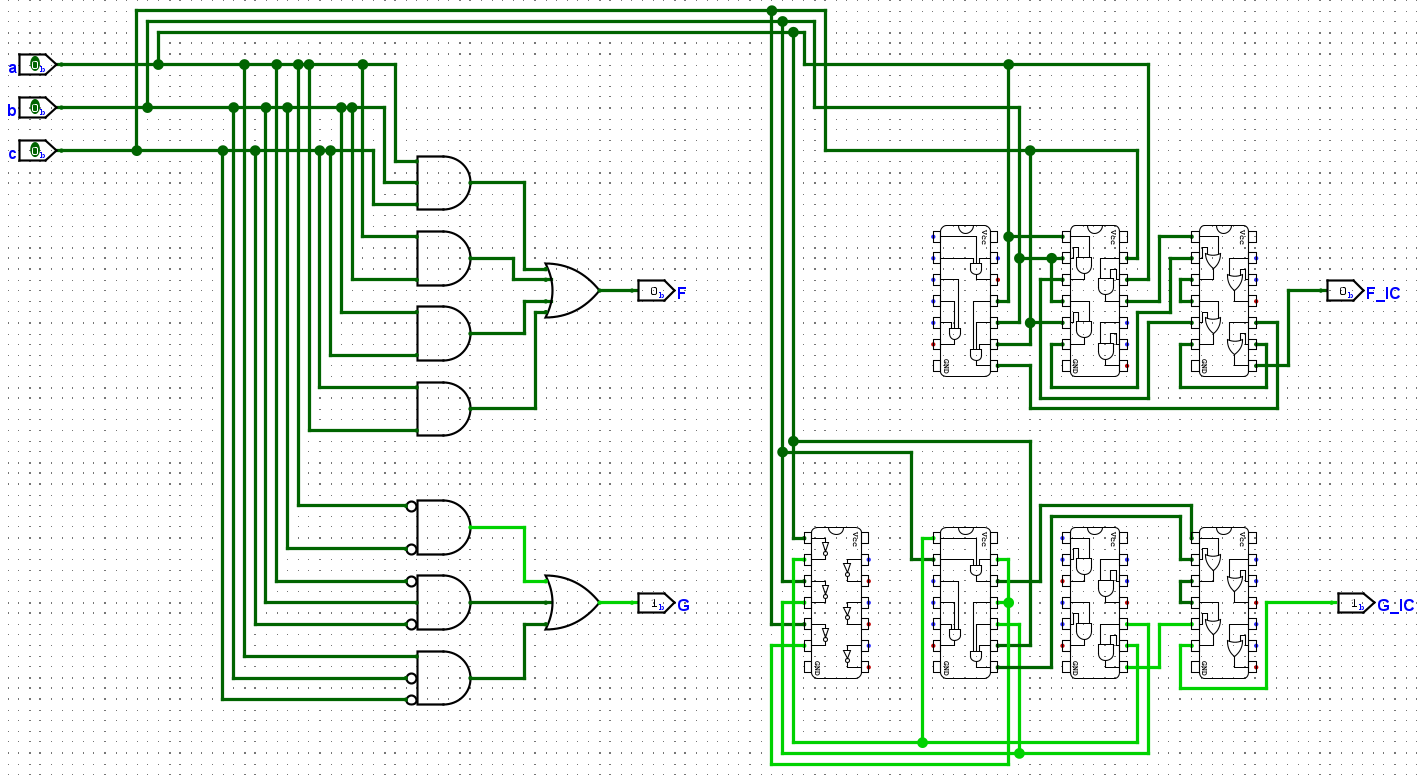
\includegraphics[width=\textwidth]{./images/circuit1.png}
    \caption{Implementations of boolean functions $F$ and $G$ using only logic gates and only 74xx series ICs.}
\end{figure}

ICs used in the implementation of boolean function $F$:
\begin{itemize}
    \item 7408 quad 2-input AND gate
    \item 7411 triple 3-input AND gate
    \item 7432 quad 2-input OR gate
\end{itemize}

\noindent ICs used in the implementation of boolean function $G$:
\begin{itemize}
    \item 7404 hex inverter
    \item 7408 quad 2-input AND gate
    \item 7411 triple 3-input AND gate
    \item 7432 quad 2-input OR gate
\end{itemize}

\subsection{Part 2}
For the pure logic gate implementations, we will assume a 22 nanosecond delay for each AND, OR, and NOT gate. 
The propagation delays for the 74xx series ICs are as follows:
\begin{itemize}
    \item 7404: 22 ns
    \item 7408: 22 ns
    \item 7411: 22 ns
    \item 7432: 22 ns
\end{itemize}

\noindent Thus, the propagation delays for the implementations of $F$ and $G$ are as follows:

\begin{itemize}
    \item $F$ (logic gates): 22 ns + 22 ns = 44 ns
    \item $G$ (logic gates): 22 ns + 22 ns + 22 ns = 66 ns
    \item $F$ (74xx series ICs): 22 ns + 22 ns = 44 ns
    \item $G$ (74xx series ICs): 22 ns + 22 ns + 22 ns = 66 ns
\end{itemize}

\subsection{Part 3}
Switching characteristics of 7404 hex inverter at Vcc = 5V and 25\degree C: \\
\begin{tabular} {|c|c|c|c|c|c|c|}
    \hline
    Symbol & Parameter & Conditions & Min & Typ & Max & Units \\
    \hline
    tplh & Propagation Delay Time LOW-to-HIGH Level Output & Cl=15pF Rl=400R & & & 22 & ns \\
    tphl & Propagation Delay Time HIGH-to-LOW Level Output & Cl=15pF Rl=400R & & & 15 & ns \\
    \hline
\end{tabular}
\\ \\ \\
Switching characteristics of 7408 quad 2-input AND gate at Vcc = 5V and 25\degree C: \\
\begin{tabular} {|c|c|c|c|c|c|c|}
    \hline
    Symbol & Parameter & Conditions & Min & Typ & Max & Units \\
    \hline
    tplh & Propagation Delay Time LOW-to-HIGH Level Output & Cl=15pF Rl=400R & & & 22 & ns \\
    tphl & Propagation Delay Time HIGH-to-LOW Level Output & Cl=15pF Rl=400R & & & 15 & ns \\
    \hline
\end{tabular}
\\ \\ \\
Switching characteristics of 7411 triple 3-input AND gate at Vcc = 5V and 25\degree C: \\
\begin{tabular} {|c|c|c|c|c|c|c|}
    \hline
    Symbol & Parameter & Conditions & Min & Typ & Max & Units \\
    \hline
    tplh & Propagation Delay Time LOW-to-HIGH Level Output & Cl=15pF Rl=400R & & & 22 & ns \\
    tphl & Propagation Delay Time HIGH-to-LOW Level Output & Cl=15pF Rl=400R & & & 15 & ns \\
    \hline
\end{tabular}
\\ \\ \\
Switching characteristics of 7432 quad 2-input OR gate at Vcc = 5V and 25\degree C: \\
\begin{tabular} {|c|c|c|c|c|c|c|}
    \hline
    Symbol & Parameter & Conditions & Min & Typ & Max & Units \\
    \hline
    tplh & Propagation Delay Time LOW-to-HIGH Level Output & Cl=15pF Rl=400R & & & 22 & ns \\
    tphl & Propagation Delay Time HIGH-to-LOW Level Output & Cl=15pF Rl=400R & & & 15 & ns \\
    \hline
\end{tabular}

\section{Problem 2}

\subsection{Part 1}
\begin{enumerate}
    \item The number of input bits is 10 since there are 10 cars with switches.
    \item We will need 7 output bits for the 7-segment display. We do not need to use the 8th decimal point input, since we have 10 cars represented from 0 to 9.
    \item We will need a 4-bit data bus between the encoder and decoder, since $\lceil \log_2 10 \rceil = 4$.
\end{enumerate}

\end{document}
